% This is the Reed College LaTeX thesis template. Most of the work
% for the document class was done by Sam Noble (SN), as well as this
% template. Later comments etc. by Ben Salzberg (BTS). Additional
% restructuring and APA support by Jess Youngberg (JY).
% Your comments and suggestions are more than welcome; please email
% them to cus@reed.edu
%
% See http://web.reed.edu/cis/help/latex.html for help. There are a
% great bunch of help pages there, with notes on
% getting started, bibtex, etc. Go there and read it if you're not
% already familiar with LaTeX.
%
% Any line that starts with a percent symbol is a comment.
% They won't show up in the document, and are useful for notes
% to yourself and explaining commands.
% Commenting also removes a line from the document;
% very handy for troubleshooting problems. -BTS

% As far as I know, this follows the requirements laid out in
% the 2002-2003 Senior Handbook. Ask a librarian to check the
% document before binding. -SN

%%
%% Preamble
%%
% \documentclass{<something>} must begin each LaTeX document
\documentclass[12pt,twoside,openany]{reedthesis}
% Packages are extensions to the basic LaTeX functions. Whatever you
% want to typeset, there is probably a package out there for it.
% Chemistry (chemtex), screenplays, you name it.
% Check out CTAN to see: http://www.ctan.org/
%%

\usepackage{setspace}
\usepackage{graphicx,latexsym}
\usepackage{amsmath}
\usepackage{amssymb,amsthm}
%\usepackage{longtable,booktabs,setspace}
\usepackage{longtable,booktabs,setspace, array}
\usepackage{chemarr} %% Useful for one reaction arrow, useless if you're not a chem major
\usepackage[hyphens]{url}
% Added by CII
\usepackage{hyperref}
\usepackage{lmodern}
\usepackage{float}
\floatplacement{figure}{H}
% End of CII addition
\usepackage{rotating}
% Next line commented out by CII
%%% \usepackage{natbib}
% Comment out the natbib line above and uncomment the following two lines to use the new
% biblatex-chicago style, for Chicago A. Also make some changes at the end where the
% bibliography is included.
%\usepackage{biblatex-chicago}
%\bibliography{thesis}


% Added by CII (Thanks, Hadley!)
% Use ref for internal links
\renewcommand{\hyperref}[2][???]{\autoref{#1}}
\def\chapterautorefname{Chapter}
\def\sectionautorefname{Section}
\def\subsectionautorefname{Subsection}
% End of CII addition

% Added by CII
\usepackage{caption}
\captionsetup{width=5in}
% End of CII addition

% \usepackage{times} % other fonts are available like times, bookman, charter, palatino

% Syntax highlighting #22

% To pass between YAML and LaTeX the dollar signs are added by CII
\title{Regime Detection Measures for the Practical Ecologist}
\author{Jessica L. Burnett}
% The month and year that you submit your FINAL draft TO THE LIBRARY
\date{2019}
% \division{}
\advisor{Craig R. Allen}
\department{School of Natural Resources}
\institution{University of Nebraska-Lincoln}
\degree{Doctor of Philosophy}
%If you have two advisors for some reason, you can use the following
% Uncommented out by CII
\altadvisor{Dirac Twidwell}
% End of CII addition

%%% Remember to use the correct department!
% if you're writing a thesis in an interdisciplinary major,
% uncomment the line below and change the text as appropriate.
% check the Senior Handbook if unsure.
%\thedivisionof{The Established Interdisciplinary Committee for}
% if you want the approval page to say "Approved for the Committee",
% uncomment the next line
%\approvedforthe{Committee}

% Added by CII
%%% Copied from knitr
%% maxwidth is the original width if it's less than linewidth
%% otherwise use linewidth (to make sure the graphics do not exceed the margin)
\makeatletter
\def\maxwidth{ %
  \ifdim\Gin@nat@width>\linewidth
    \linewidth
  \else
    \Gin@nat@width
  \fi
}
\makeatother

\renewcommand{\contentsname}{Table of Contents}
% End of CII addition

\setlength{\parskip}{0pt}

% Added by CII

\providecommand{\tightlist}{%
  \setlength{\itemsep}{0pt}\setlength{\parskip}{0pt}}

\Acknowledgements{
Graduate school itself isn't hard, but the journey is. I have a lot of
people and institutions to thank for their emotional, intellectual,
financial, and other support. I wish to first highlight how
\textbf{great it was to be a graduate student at this university and in
the School of Natural Resources}. UNL has provided tremendous support at
all levels of the university. Although I am not a fan of Nebraska's
climate, I highly recommend this school to prospective students. I thank
my supervisors, Craig Allen and Dirac Twidwell, for providing me with
this amazing opportunity and for supporting my growth as an independent
researcherm and my committee members, Craig Allen, David Angeler, John
De Long, Dirac Twidwell, and Drew Tyre for their support and advisement,
but especially for their comprehensive examination--I found this process
transformative, albeit very stress inducing. I also wish to thank Dirac
for his comprehensive exam questions--I never knew how much I didn't
know until I studied your recommendations. I also thank Craig for
supporting my efforts to study and conduct research outside of our
immediate geographical settings. Studying at the International Institute
for Applied Systems Analysis was an amazing opportunity! I thank Brian
Fath and Elena Rovenskaya for their advisement, members of the Applied
Systems Analysis research group for their feedback on my research, and
to the postdocs and YSSPers. I would like to especially thank some of
the amazing and brilliant \textbf{female scientists} in my life for
their encouragement: Jane Anderson, Karen Bailey, Hannah Birge, Mary
Bomberger Brown, Tori Donovan, Brittany Dueker, Allie Schiltmeyer, Katie
Sieving, Erica Stuber, Becky Wilcox, Carissa Wonkka, and Lyndsie Wszola.
I thank these women and others for their contributions to my
professional development: David Angeler, Christie Bahlai, Mary Bomberger
Brown, John Carroll, Jenny Dauer, John DeLong, Tarsha Eason, Brian Fath,
Ahjond Garmestani, Chris Lepczyk, Frank La Sorte, Chai Molina, Zac
Warren, Hao Ye and Peter Zebrowski. I owe thanks to Craig Allen and
Kevin Pope for entertaining my many hours of discussion (interrogation?)
regarding federal employment. I also thank fellow graduate students whom
I hope I have forged strong and lasting connections: Hannah Birge, Tori
Donovan, Caleb Roberts, Allie Schiltmeyer, and Lyndsie Wszola I am one
of the many graduate students afflicted with mental health
``disorders''. I am first grafteful to one friend (H) who unknowingly
destigmatized mental health in my mind and wihtout whom I may not have
sought treatment. I applaud students and faculty who have been outspoken
regarding mental health related issues, and I am indebtted to my general
practitioner and mental health advocate, Terry Thomas M.A., M.S.N.,
A.P.R.N.\\
\emph{Financial support}. This research was funded by the U.S.
Department of Defense's Strategic Environmental Research and Development
Program (project ID: RC-2510). The University of Nebraska-Lincoln (UNL)
has been highy supportive in my doctoral studies and reserach. I am
grateful for the generous of donors to the University of Nebraska
Foundation, which provided me with two prestigious supplemental
fellowships: Fling and Othmer. I also thank the Nelson Family (Nelson
Memorial Fellowship) and the Institute of Agriculture and Natural
Resources, who funded large portions of my academic and research-related
travel. I thank the School of Natural Resources for their financial
support in my conference travel. The U.S. National Academy of Sciences
generously funded part of my travel to the International Institute for
Applied Systems Analysis (IIASA). This financial support provided me not
only with invaluabe opportunities to attend and present at national and
international conferences and workshops, conduct research abroad, and
network--this funding alleviated some financial pressures associated
with graduate school which allowed a more refined focus on my
dissertation research. The opportunities and experiences provided to me
by each funding source were amazing, thank you. Finally, to my partner
of eight years--Schultzie--thank you for everything. Just kidding, thank
you, Nat Price, you are amazing.
}

\Dedication{
To the end-users and researchers frustrated with jargon and lack of
practical utility of ecological models and metrics. And to Mike Moulton,
without whose support and encouragement many years ago two advanced
degrees would likely not have been possible.
}

\Preface{

}

\Abstract{

}

% End of CII addition
%%
%% End Preamble
%%
%
\begin{document}

% Everything below added by CII
  \maketitle

\frontmatter % this stuff will be roman-numbered
\pagestyle{empty} % this removes page numbers from the frontmatter
  \begin{acknowledgements}
    Graduate school itself isn't hard, but the journey is. I have a lot of
    people and institutions to thank for their emotional, intellectual,
    financial, and other support. I wish to first highlight how
    \textbf{great it was to be a graduate student at this university and in
    the School of Natural Resources}. UNL has provided tremendous support at
    all levels of the university. Although I am not a fan of Nebraska's
    climate, I highly recommend this school to prospective students. I thank
    my supervisors, Craig Allen and Dirac Twidwell, for providing me with
    this amazing opportunity and for supporting my growth as an independent
    researcherm and my committee members, Craig Allen, David Angeler, John
    De Long, Dirac Twidwell, and Drew Tyre for their support and advisement,
    but especially for their comprehensive examination--I found this process
    transformative, albeit very stress inducing. I also wish to thank Dirac
    for his comprehensive exam questions--I never knew how much I didn't
    know until I studied your recommendations. I also thank Craig for
    supporting my efforts to study and conduct research outside of our
    immediate geographical settings. Studying at the International Institute
    for Applied Systems Analysis was an amazing opportunity! I thank Brian
    Fath and Elena Rovenskaya for their advisement, members of the Applied
    Systems Analysis research group for their feedback on my research, and
    to the postdocs and YSSPers. I would like to especially thank some of
    the amazing and brilliant \textbf{female scientists} in my life for
    their encouragement: Jane Anderson, Karen Bailey, Hannah Birge, Mary
    Bomberger Brown, Tori Donovan, Brittany Dueker, Allie Schiltmeyer, Katie
    Sieving, Erica Stuber, Becky Wilcox, Carissa Wonkka, and Lyndsie Wszola.
    I thank these women and others for their contributions to my
    professional development: David Angeler, Christie Bahlai, Mary Bomberger
    Brown, John Carroll, Jenny Dauer, John DeLong, Tarsha Eason, Brian Fath,
    Ahjond Garmestani, Chris Lepczyk, Frank La Sorte, Chai Molina, Zac
    Warren, Hao Ye and Peter Zebrowski. I owe thanks to Craig Allen and
    Kevin Pope for entertaining my many hours of discussion (interrogation?)
    regarding federal employment. I also thank fellow graduate students whom
    I hope I have forged strong and lasting connections: Hannah Birge, Tori
    Donovan, Caleb Roberts, Allie Schiltmeyer, and Lyndsie Wszola I am one
    of the many graduate students afflicted with mental health
    ``disorders''. I am first grafteful to one friend (H) who unknowingly
    destigmatized mental health in my mind and wihtout whom I may not have
    sought treatment. I applaud students and faculty who have been outspoken
    regarding mental health related issues, and I am indebtted to my general
    practitioner and mental health advocate, Terry Thomas M.A., M.S.N.,
    A.P.R.N.\\
    \emph{Financial support}. This research was funded by the U.S.
    Department of Defense's Strategic Environmental Research and Development
    Program (project ID: RC-2510). The University of Nebraska-Lincoln (UNL)
    has been highy supportive in my doctoral studies and reserach. I am
    grateful for the generous of donors to the University of Nebraska
    Foundation, which provided me with two prestigious supplemental
    fellowships: Fling and Othmer. I also thank the Nelson Family (Nelson
    Memorial Fellowship) and the Institute of Agriculture and Natural
    Resources, who funded large portions of my academic and research-related
    travel. I thank the School of Natural Resources for their financial
    support in my conference travel. The U.S. National Academy of Sciences
    generously funded part of my travel to the International Institute for
    Applied Systems Analysis (IIASA). This financial support provided me not
    only with invaluabe opportunities to attend and present at national and
    international conferences and workshops, conduct research abroad, and
    network--this funding alleviated some financial pressures associated
    with graduate school which allowed a more refined focus on my
    dissertation research. The opportunities and experiences provided to me
    by each funding source were amazing, thank you. Finally, to my partner
    of eight years--Schultzie--thank you for everything. Just kidding, thank
    you, Nat Price, you are amazing.
  \end{acknowledgements}

  \hypersetup{linkcolor=black}
  \setcounter{tocdepth}{2}
  \tableofcontents

  \listoftables

  \listoffigures

  \begin{dedication}
    To the end-users and researchers frustrated with jargon and lack of
    practical utility of ecological models and metrics. And to Mike Moulton,
    without whose support and encouragement many years ago two advanced
    degrees would likely not have been possible.
  \end{dedication}
\mainmatter % here the regular arabic numbering starts
\pagestyle{fancyplain} % turns page numbering back on
% \doublespacing{} % Trying to set spacing between lines in body
\linespread{1} % Trying to set spacing between lines in body

\chapter{thesisdown::thesis\_gitbook:
default}\label{thesisdownthesis_gitbook-default}

Placeholder

Identifying abrupt changes in the structure and functioning of systems,
or system regime shifts, in ecological and social-ecological systems
leads to an understanding of relative and absolute system resilience.
Resilience is an emergent phenomenon of complex social-ecological
systems, and is the ability of a system to absorb disturbance without
reorganizing into a new state, or regime. Resilience science provides a
framework and methodology for quantitatively assessing the capacity of a
system to maintain its current trajectory (or to stay within a certain,
and often desirable regime). If and when a system's resilience is
exceeded, it crosses a threshold and enters into an alternate regime (or
undergoes a regime shift).\\
I will use Fisher Information to detect regime shifts in time and space
using avian community data obtained from the North American Breeding
Bird Survey within the area east of the Rockies and west of the
Mississippi River. Fisher Information is a technique that captures the
dynamic of a system, and this metric will be calculated about a suite of
bird species abundances aggregated to the route level for all possible
time periods. Transmutation (aggregation error) about inclusion or
exclusion of certain bird species, functional groups, and guilds will be
analyzed. Efforts have been made to develop early warning indicators of
regime shifts in ecosystems, however, for most ecosystems there is great
uncertainty in predicting the risk of a regime shift, regarding both
when and how long it will take to happen and if it can be recognized
early enough to be avoided when desired. We will complement the use of
Fisher Information with multiple discontinuity analyses about body mass
distributions at the route-level to achieve the aim of identifying
individual species that best serve as early-warning indicators of regime
shifts. For those species found on the edges of body mass aggregations,
we test the hypothesis that the background variance in their abundances
(on Breeding Bird Survey routes) will increase more than those not
observed at the edge of discontinuity aggregations. Identification of
early-warning indicators of regime shifts in ecological systems allows
management efforts to focus on a single or a small number of species
that inform us about ecosystem resilience and trajectory.\\
These methods transcend the primary objective of the Breeding Bird
Survey (to monitor population trends) and use this expansive dataset in
such a way that information about ecosystem order, trajectory, and
resilience emerge. Here, we utilize an expansive dataset (the Breeding
Bird Survey) to make broad-scale estimations and predictions about
ecosystem resilience, regime status and trajectory, and ecosystem
sustainability. Identification of regime shifts and early-warning
indicator species may afford us the ability to predict system regime
shifts in time.

\chapter{Introduction}\label{intro}

Placeholder

\subsection{Dissertation structure}\label{dissertation-structure}

\section{Glossary}\label{glossary}

\chapter{A brief overview of ecological regime detection methods
methods}\label{rdmReview}

Placeholder

\section{Introduction}\label{introduction}

\section{Methods}\label{methods}

\subsection{Identifying candidate
articles}\label{identifying-candidate-articles}

\subsubsection{Web of Science}\label{web-of-science}

\subsubsection{Prior knowledge and snowball
method}\label{prior-knowledge-and-snowball-method}

\subsubsection{Google Scholar}\label{google-scholar}

\subsubsection{Additional filtering}\label{additional-filtering}

\section{Results}\label{results}

\subsection{Web of Science}\label{web-of-science-1}

\subsection{Google Scholar and prior
knowledge}\label{google-scholar-and-prior-knowledge}

\subsection{List of new methods}\label{list-of-new-methods}

\section{Discussion}\label{discussion}

\subsection{Barriers to identifying new
RDMs}\label{barriers-to-identifying-new-rdms}

\subsection{Reducing the barriers to
RDMs}\label{reducing-the-barriers-to-rdms}

\chapter{A guide to Fisher Information for Ecologists}\label{fiGuide}

Placeholder

\section{Abstract}\label{abstract}

\section{Introduction}\label{introduction-1}

\subsection{On Fisher Information}\label{on-fisher-information}

\subsection{Notation}\label{notation}

\subsection{Steps for calculating Fisher Information
(FI)}\label{steps-for-calculating-fisher-information-fi}

\subsection{Concepts behind the
calculations}\label{concepts-behind-the-calculations}

\subsubsection{\texorpdfstring{\textbf{Step 1. Probability of observing
the system in a particular state,
\(p(x)\)}}{Step 1. Probability of observing the system in a particular state, p(x)}}\label{step-1.-probability-of-observing-the-system-in-a-particular-state-px}

\subsubsection{\texorpdfstring{\textbf{Step 2.} Distance traveled by the
system,
\(s\)}{Step 2. Distance traveled by the system, s}}\label{step-2.-distance-traveled-by-the-system-s}

\subsubsection{\texorpdfstring{\textbf{Step 3.} \(p(s)\) as a function
of the rate of change of
\(s\)}{Step 3. p(s) as a function of the rate of change of s}}\label{step-3.-ps-as-a-function-of-the-rate-of-change-of-s}

\subsubsection{\texorpdfstring{\textbf{Step 4.} Calculate the
derivatives-based Fisher
Information}{Step 4. Calculate the derivatives-based Fisher Information}}\label{step-4.-calculate-the-derivatives-based-fisher-information}

\section{Case Study}\label{case-study}

\section{Conclusions}\label{conclusions}

\section{Acknowledgements}\label{acknowledgements}

\chapter{An application of Fisher Information to spatially-explicit
avian community data}\label{fisherSpatial}

Placeholder

\section{Introduction}\label{introduction-2}

\section{Data and Methods}\label{data-and-methods}

\subsection{Data: North American Breeding Bird
Survey}\label{data-north-american-breeding-bird-survey}

\subsection{Study area}\label{study-area}

\subsubsection{Focal military base}\label{focal-military-base}

\subsubsection{Spatial sampling grid}\label{spatial-sampling-grid}

\subsection{Calculating Fisher Information
(FI)}\label{calculating-fisher-information-fi}

\subsection{Interpreting and comparing Fisher Information across spatial
transects}\label{interpreting-and-comparing-fisher-information-across-spatial-transects}

\subsubsection{Interpreting FI values}\label{interpreting-fi-values}

\subsubsection{Interpolating results across spatial
transects}\label{interpolating-results-across-spatial-transects}

\subsubsection{Spatial correlation of Fisher
Information}\label{spatial-correlation-of-fisher-information}

\section{Results}\label{results-1}

\subsection{Fisher Information across spatial
transects}\label{fisher-information-across-spatial-transects}

\subsection{Spatial correlation of Fisher
Information}\label{spatial-correlation-of-fisher-information-1}

\section{Discussion}\label{discussion-1}

\subsection{Efficacy of Fisher Information as a spatial
RDM}\label{efficacy-of-fisher-information-as-a-spatial-rdm}

\chapter{Data Quality Impacts on Regime Detection
Measures}\label{resampling}

Placeholder

\section{Introduction}\label{introduction-3}

\section{Methods}\label{methods-1}

\subsection{Study system and data}\label{study-system-and-data}

\section{Results}\label{results-2}

\section{Discussion}\label{discussion-2}

\section{Ackowledgements}\label{ackowledgements}

\chapter{\texorpdfstring{Velocity (\emph{v}): rate-of-change of system
trajectory as a potential indicator of abrupt
change}{Velocity (v): rate-of-change of system trajectory as a potential indicator of abrupt change}}\label{velocity}

\section{Introduction}\label{introduction-4}

Dimension reduction techniques and RDms blablbah In this Chapter I
describe the steps for calculating a `new' metric, \textbf{system
velocity}, for reducing the dimensionality and identifying abrupt shifts
in high dimensional data. Although this is the first instance of this
calculation to, alone, be suggested as a regime detection metric, it has
been used as part of a larger series of calculations of the Fisher
Information metric {[}see \ref{fiGuide}{]}, first introduced in Fath,
Cabezas, \& Pawlowski (2003). Below, I describe the steps for
calculating system velocity, simply defined as the cumulative sum of the
squared change in all state variables over a period of time.

\section{About the toy system}\label{about-the-toy-system}

Consider a system (Fig. \ref{fig:sysEx}) with \(N\) state variables
(\(x_i\)), with observations taken at time points, \(t\). System
velocity is calculated as the cumulative sum over time period \(t_0\) to
\(t_j\), as the total change in all state variables, \{\(x_1 ...x_N\)\},
between two adjacent time points, e.g., \(t_j\) and \(t_{j+1}\), denoted
\(t_{j,j+1}\). I use a simple, two-variable system to demonstrate the
calculation of each step below. The system comprises variables \(x_1\)
and \(x_2\), with observations occurring at each time point
\(t = {1,2,3,...100}\).
\begin{figure}

{\centering 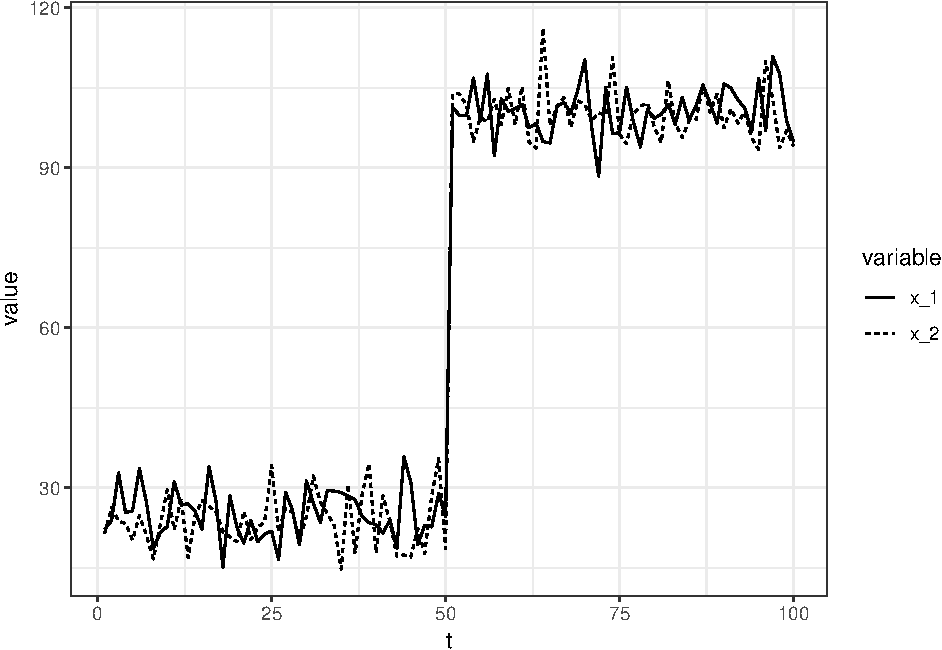
\includegraphics[width=0.95\linewidth]{_myDissertation_files/figure-latex/sysEx-1} 

}

\caption{The 2-variable toy system used to demonstrate steps for calculating system velocity. Each variable, $x$, is drawn from a normal distribution with means that change at $t = 50$. State variables have constant variance $\sigma = 5$. }\label{fig:sysEx}
\end{figure}
\section{\texorpdfstring{Steps for calculating system velocity,
\emph{v}}{Steps for calculating system velocity, v}}\label{steps-for-calculating-system-velocity-v}

First, we calculate the change in each state variable, \(x_i\), between
two adjacent points in time, \(t_j\) and \(t_{j+1}\), such that the
difference, \(x_{t_{j+1}} - x_{t_j}\) is assigned to the latter time
point, \(t_{j+1}\). For example, in our toy data, we use observations at
time points \(t = 1\) \& \(t=2\) (Fig. \ref{fig:sysEx2}). For all
examples in this chapter, the state variables \(x_1\) and \(x_2\) were
drawn from a normal distribution (using function \emph{rnorm}), with
parameters \(\bar{x}_i\) (mean) and \(\sigma_i\) (sd) for 100 time
steps, \(t\). The regime shift occurs at \(t=50\), where a shift in
either or both \(\bar{x}_i\) or \(\sigma_i\).

\subsubsection{\texorpdfstring{Step 1:
\(\Delta x_i\)}{Step 1: \textbackslash{}Delta x\_i}}\label{step-1-delta-x_i}

The first step in calculating \(v\) is to obtain the change in values
for each state variables, \(x_1\) and \(x_2\) between two consecutive
time points (e.g., from \(t=1\) to \(t=2\):
\begin{equation}
\begin{array}{rcr}
\Delta x_1 = x_{1_{t=2}} - x_{1_{t=1}} \\
\Delta x_2 = x_{2_{t=2}} - x_{1_{t=1}}
  \end{array}
\label{eq:diffX}
\end{equation}\begin{figure}
{\centering 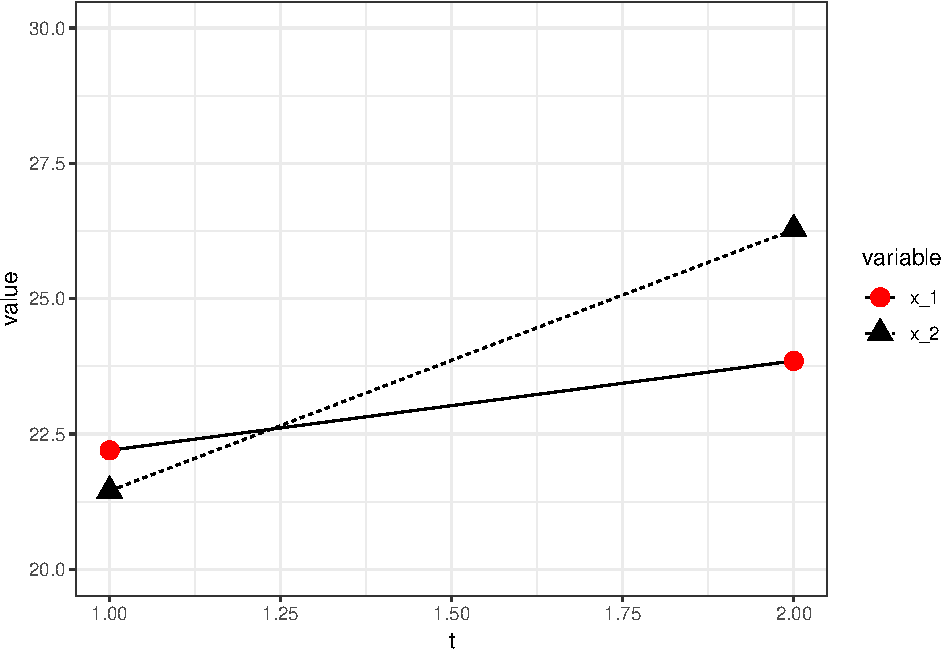
\includegraphics[width=0.95\linewidth]{_myDissertation_files/figure-latex/sysEx2-1} 

}

\caption{Data used to calculate velocity at the first two time points, $t_1$ and $t_2$.}\label{fig:sysEx2}
\end{figure}
\subsubsection{\texorpdfstring{Step 2:
\(\sqrt(\sum_i^N\Delta x_1^2)\)}{Step 2: \textbackslash{}sqrt(\textbackslash{}sum\_i\^{}N\textbackslash{}Delta x\_1\^{}2)}}\label{step-2-sqrtsum_indelta-x_12}

After calculating the differences for each state variable, we will next
calculate the total change in the system over the time elapsed,
following Pythagora's theorem,
\begin{equation}
 X_1^2 + X_2^2 = s^2 
  \label{eq:pythagorean}
\end{equation}
where \(s\) represents the total change in the system, and \(X_1\) and
\(X_2\) represent the changes in all state variables
(\(x_{i_{t=2}} - x_{i_{t=1}}\)). We achieve this by first squaring the
differences obtained in Eq. \eqref{eq:diffX}:
\begin{equation}
\begin{array}{rcr}
(x_{1_{t=2}} - x_{1_{t=1}})^2  \\
(x_{2_{t=2}} - x_{2_{t=1}})^2 
\end{array}
  \label{eq:diffXsq}
\end{equation}
\subsubsection{\texorpdfstring{Step 3: Use Pythagorean theorem to
isolate
\(s\)}{Step 3: Use Pythagorean theorem to isolate s}}\label{step-3-use-pythagorean-theorem-to-isolate-s}

Next, we isolate \(s\) in Eq. \eqref{eq:pythagorean}, capturing the total
change in all state variables into a single measure by taking the 2nd
root of the squared sums of all \(x\):
\begin{equation}
\begin{array}{rcr}
\sum_{i=1}^{N} \Delta {x_i} = \sum_{i=1}^{N}(x_{t_{i+1}} - x_{t_i})^2 \\ 
\ = \Delta s \\ 
\ = \sqrt([x_{1_{t=2}} - x_{1_{t=1}}]^2 + [x_{2_{t=2}} - x_{2_{t=1}}]^2)
\end{array}
\label{eq:diffXsq2}
\end{equation}
We now have a single measure, \(\Delta s\) (Eq. \eqref{eq:diffXsq2}), for
each pair of time points in our \(N\)-dimensional system. It is obvious
that \(\Delta s\) will always be a positive value, since we took the 2nd
root of a squared value. Although discussed in a later section, it is
important to note that this value is not unitless--that is, our example
system takes on the units of our state variables, \(x_1\) and \(x_2\).
Because we are interested in identifying abrupt changes in the entire
system, we calculate the cumulative sum of \(\Delta s\) at every time
point, such that:
\begin{equation}
s = \sum_{t=1}^T \Delta s
\label{eq:s}
\end{equation}
\subsubsection{\texorpdfstring{Step 4: Calculate velocity, \(v\) (or
\(\frac {\Delta s}{\Delta t}\))}{Step 4: Calculate velocity, v (or \textbackslash{}frac \{\textbackslash{}Delta s\}\{\textbackslash{}Delta t\})}}\label{step-4-calculate-velocity-v-or-frac-delta-sdelta-t}

Finally, we calculate the \textbf{system velocity}, \(v\) (or
\(\frac{\Delta s}{\Delta t}\)), by first calculating the change in \(s\)
(Eq. \eqref{eq:s}), and then divide by the total time elapsed between
consecutive sampling points:
\begin{equation}
 v = \frac {s_{t+1}-s_{t}}{\Delta t} 
\label{eq:velocity}
\end{equation}\begin{figure}
{\centering 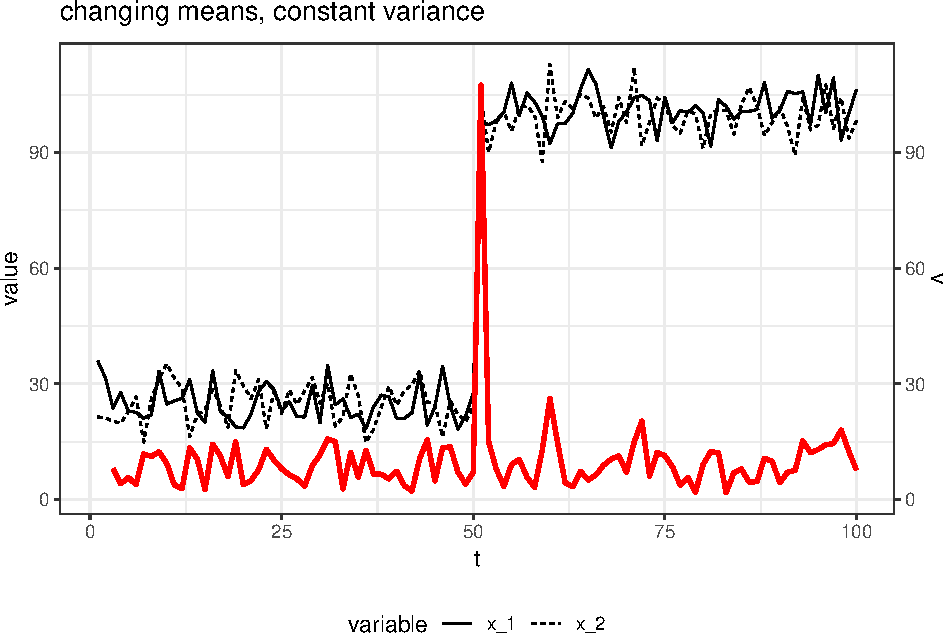
\includegraphics[width=0.95\linewidth]{_myDissertation_files/figure-latex/velocSysEx1-1} 

}

\caption{System change ($s$) and velocity ($v$) of the model system over the time period. Constant means ($\bar{x}_{pre}=25$, $\bar{x}_{post}=10$) and sharp change in variance for both state variables, $\sigma =5$.}\label{fig:velocSysEx1}
\end{figure}
The steps for calculating velocity {[}Eq. \eqref{eq:velocity}{]} are
demonstrated using the first five time points of our toy system (Fig.
\ref{fig:sysEx}) in Table \ref{tab:distTab}.

\section{\texorpdfstring{Velocity \emph{v} performance under varying
mean and variance in the toy
system}{Velocity v performance under varying mean and variance in the toy system}}\label{velocity-v-performance-under-varying-mean-and-variance-in-the-toy-system}

I simulated 10,000 random draws of the toy system, which experiences a
rapid shift at \(t = 50\), while varying two each of the following
system paramters at the regime shift: \(\bar{x}_1\), increased the mean
value of \(x_1\) \(\sigma_1\), change in variance of \(x_1\) Simulations
consisted of 10,000 random samples drawn from the normal distribution
for each paramter, I randomly drew the toy system samples 10,000 times
under increasing values of \(\bar{x}_1\) and \(\sigma_1\). To identify
patterns in the influence of paramter values on velocity, I present the
mean values of \(v\) across all simulations, with confidence intervals
of \(\pm 2\) standard deviations. As mentione above, the state variables
\(x_1\) and \(x_2\) were drawn from a normal distribution (using
function \emph{rnorm}), with parameters \(\bar{x}_i\) (mean) and
\(\sigma_i\) (sd) for 50 time steps, \(t\).

\subsubsection{Varying post-shift mean}\label{varying-post-shift-mean}

I examined the influence of the magnitude of change in \(x_1\) in the
period before (pre; \(t <50\)) and after (post; \(t \geq 50\)) by
varying the mean parameter, \(\bar{x}_1\) in the set
\(W=\{25,30,35,...100 \}\) (Figs. \ref{fig:simVplot1},\ref{simVplot2}).
As expected, the magnitude of \(v\) increased linearly as the total
difference between \(\bar{x}_{1_{pre}}\) and \(\bar{x}_{1_{post}}\)
increased (\ref{fig:simVplot2}). This is not surprising, as \(s\)
increases as the total change in abundance across the entire sytem
increases (Eq. \eqref{eq:s}), therefore, the potential maximum of \(v\)
also increases. This may indicate that \(v\), while capable of
identifying large shifts in data structure, may not pick up subtle
changes (i.e.~lower effect sizes).
\begin{figure}

{\centering 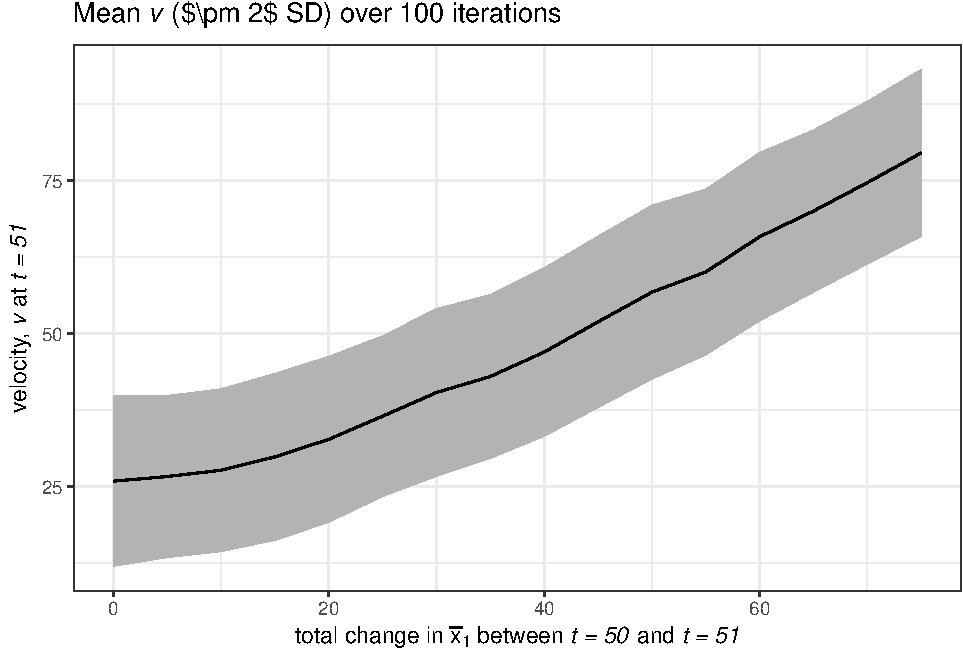
\includegraphics[width=0.95\linewidth]{_myDissertation_files/figure-latex/simVplot2-1} 

}

\caption{Change in velocity ($v$) as the total change in the mean value of $\bar{x}_{2_{t=50}}$ over 10,000 simulations. A regime shift was induced at $t=50$ with constant varoance $\sigma = 5$, $\bar{x}_2 = 25$ when $t<50$,  and changes in variable mean values, $\bar{x}_2 = 50$ when $t \geq 50$, $\bar{x}_1 = 25$ when $t<50$.}\label{fig:simVplot2}
\end{figure}
\subsubsection{Varying post-shift
variance}\label{varying-post-shift-variance}

In the previous example, variance was constant before and after the
shift at \(t=50\). To determine whether the signal emitted by \(v\) at
the regime shift is lost with increasing variance, I varied the variance
parameter, \(\sigma_1\) in the set \(W = \{1,2,3,...25 \}\). The
variance for both state variables prior to the regime shift,
\(\sigma_1\) and \(\sigma_2\), was 5, with the change occurring in
\(\sigma_1{_{post}}\). Sytem velocity \(v\) appears senstive to
increases in the variance at the point of the regime shift (Figs.
\ref{fig:simVarplot}, \ref{fig:simVarplot2}). This extreme sensitivity
of \(v\) to \(\sigma{_{post}}\) (Fig. \ref{fig:simVarplot2}) is
unsurprising, given the fact that, without smoothing the derivatives,
the tangential speed of a `noisy' variable will always be noisy itself
(see Figs. \ref{velocitySysEx1}, \ref{velocitySysEx2},
\ref{velocitySysEx3}, \ref{velocitySysEx4}).
\begin{figure}

{\centering 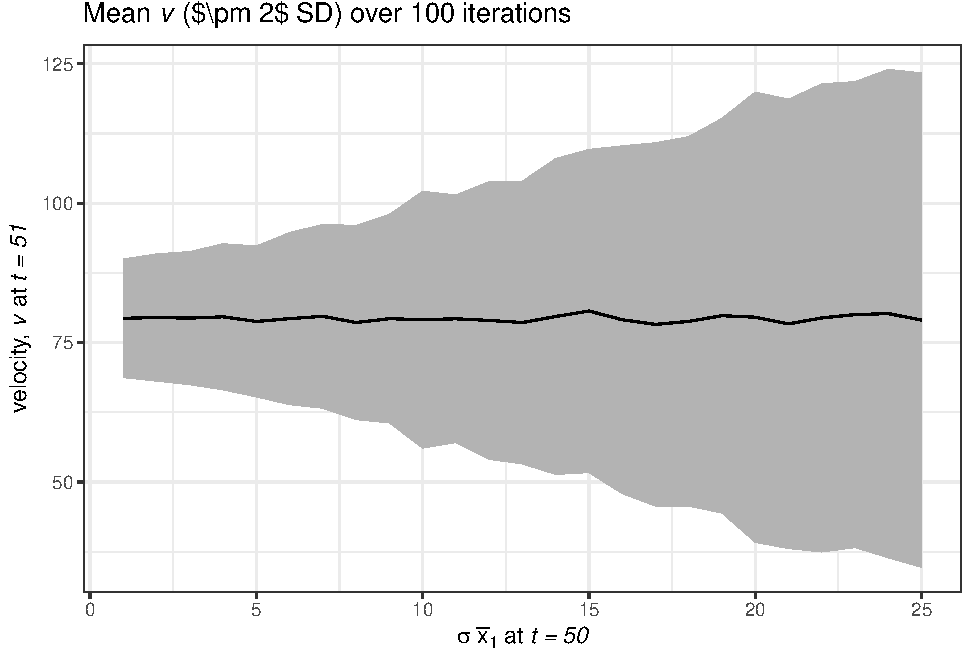
\includegraphics[width=0.95\linewidth]{_myDissertation_files/figure-latex/simVarPlot2-1} 

}

\caption{Average ($\pm 2$ SD) velocity ($v$) woresens as the variance of $\bar{x}_{2_{t=50 (post)}}$ (post shift) increases. $\bar{x}_{1_{pre}} = 25$, $\bar{x}_{1_{post}} = 100$, $\bar{x}_{2_{pre}} = 25$, $\bar{x}_{2_{post}} = 50$, $\sigma_{1_{pre}} = 5$, $\sigma_{2_{pre,post}} = 5$}\label{fig:simVarPlot2}
\end{figure}
\subsubsection{\texorpdfstring{Smoothing the data prior to calculating
\emph{v}}{Smoothing the data prior to calculating v}}\label{smoothing-the-data-prior-to-calculating-v}

To ameliorate the influence of noise (e.g.~Fig. \ref{simVarPlot}) on the
regime shift signal in \(v\), I used linear approximation techniques in
attempt to smooth the velocity (derivatives). I used the function
\emph{stats::approx} to interpolate values of \(x_1\) and \(x_2\) to
regularly-spaced time points in the set \(t=\{1:100\}\), and then
calculated \(v\) as described in the steps above (Eqs.
\eqref{eq:diffX}:\eqref{eq:velocity}). Increasing the number of points
(\(t\)) at which the original state variables were smoothed did not
influence the amount of noise surrounding the signal of the regime shift
(at \(t=50\)) in system velocity, \(v\) (Fig. \ref{fig:smoothV}).

\section{Discussion}\label{discussion-3}

In this chapter, I described the steps for calculating a novel regime
detection metric, system velocity (\(v\)). First described in Fath et
al. (2003), \(v\) is used as a single step for caclulating a more
complicated regime detection metric, Fisher Information (see also
Chapter \ref{fiGuide}). System velocity is arguably simple to calculate,
as shown in this chapter, captures the total change in system variables
under a variety of mean and variance conditions. The metric does not,
however, perform well as variance increases (Fig. \ref{simVarPlot2}),
and smooothing the original data does not reduce the noise surrounding
this metric when variance is moderate (Fig. \ref{smoothV}).

Variance is a commonly-used indicator of ecological regime shifts (Brock
\& Carpenter (2006)), however, fails to perform when the number of
variables is \textgreater{}\textgreater{} a few. System velocity, \(v\),
may be useful in situations where the number of state variables is much
greater than a few, and appears especially useful when the magnitude of
change in one or more state variables is high (Fig.
\ref{fig:simVplot2}). For example, this method will likely identify
signals of regime shifts where the shift is defined as high species
turnover within a community.

I tested the efficacy of this metric as an indicator of abrupt change in
a two-variable system. Although a useful first step, this metric should
be considered in a multi-species context, and particularly in
community-level empirical data which is difficult to simulate. I
demonstrate a compelling case study in materials associated with my R
Package, \textbf{regimeDetectionMeasures}, and in Appendix
\ref{appPaleo} in which multiple species turnover events are apparent in
a paleodiatom community time series. In this case study, the `distance
travelled', \(s\) (Eq. \eqref{eq:diffXsq2}), clearly exhibits shifts at
points where expert opinion and species turnover (in species dominance)
agree that a large change occurred. Further, velocity, \(v\) (see
\emph{dsdt} in the package materials) indicates a large shift at only
the most predonimnant shift in the time series, perhaps due to the
metric's sensitivity to variance (Fig. \ref{fig:simVplot2}.

Further work is required to determine the utility of system velocity as
a regime detection metric, however, this chapter demonstrates that the
metric may indicate clear shifts in variable means. For multispecies
data you will typically need to reduce dimensionality before you can
proceed with analyses, for example using some sort of ordination. In
addition to examining high-dimensional and noisy data, a study of the
performance of \(v\) under conditions where few variables exhibit large
changes while many variables are relatively constant may also prove
useful. Additionally, this metric may be a useful tool for reducing the
dimensionality of high dimensional data. Although the metric loses much
information, as opposed to some dimension reduction techniques,
e.g.~Principal Components Analysis PCA, the metric is simple to
calculate (even by hand), is computationally inexpensive, and is
intuitive, unlike many clustering algorithms (e.g., Non-metric
Multidimensional Scaling NMDS). Like system velocity, methods of the
latter variety (e.g.~NMDS) require post-hoc statistical analyses to
confirm the location of clusters (or abrupt change, regime shifts),
while methods of the former variety (e.g.~PCA) retain loadings but do
not necessarily identify the locations of abrupt shifts.

\section{Supplementary Materials}\label{supplementary-materials}
\begin{figure}

{\centering 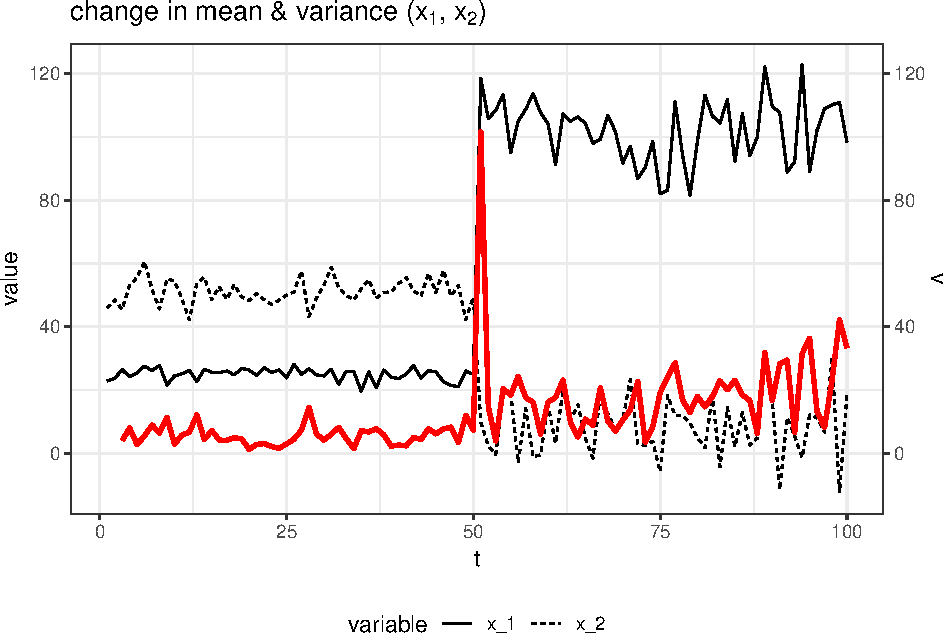
\includegraphics[width=0.95\linewidth]{_myDissertation_files/figure-latex/velocSysEx2-1} 

}

\caption{System change ($s$) and velocity ($v$) of the model system over the time period. Change in means ($\bar{x}_{1_{pre}}=25$, $\bar{x}_{1_{post}}=100$, $\bar{x}_{2_{pre}}=50$, $\bar{x}_{2_{post}}=10$) and an increase in variance ($\sigma_{1_{pre}}=2$, $\sigma_{1_{post}}=10$, $\sigma_{2_{pre}}=5$,  $\sigma_{2_{post}}=10$).}\label{fig:velocSysEx2}
\end{figure}
\begin{figure}

{\centering 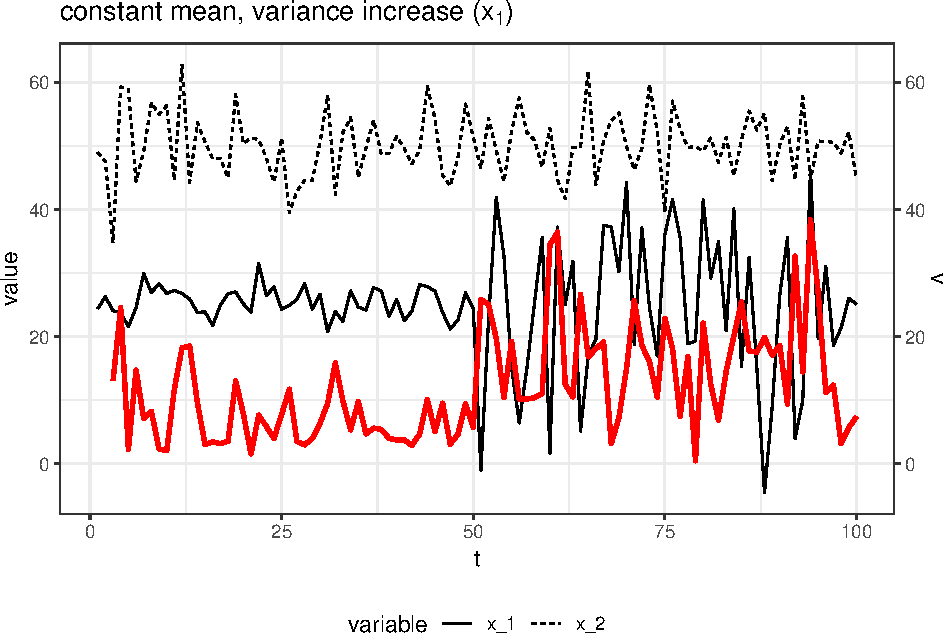
\includegraphics[width=0.95\linewidth]{_myDissertation_files/figure-latex/velocSysEx3-1} 

}

\caption{System change ($s$) and velocity ($v$) of the model system over the time period. Constant means ($\bar{x}_1=25$, $\bar{x}_2=50$) and sharp change in variance for one state variable $\sigma_{1_{pre}} = 2$, $\sigma_{1_{post}} = 12$, $\sigma_{2_{pre,post}} = 5$}\label{fig:velocSysEx3}
\end{figure}
\begin{figure}

{\centering 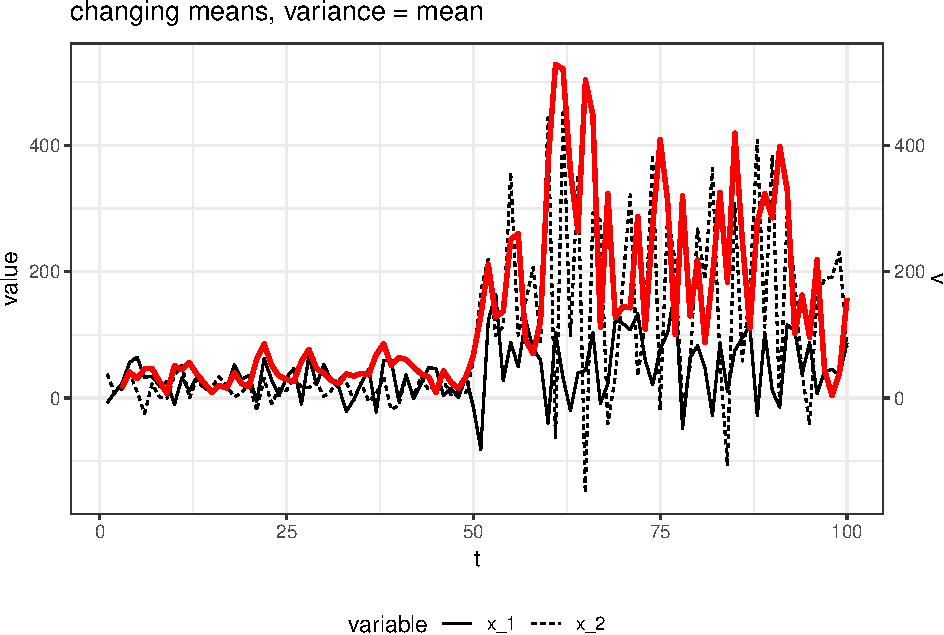
\includegraphics[width=0.95\linewidth]{_myDissertation_files/figure-latex/velocSysEx4-1} 

}

\caption{System change ($s$) and velocity ($v$) of the model system over the time period. Variance equal to mean ($\bar{x_i}=\sigma_i$), where means ($\bar{x}_{1_{pre}}=25$, $\bar{x}_{1_{post}}=50$, $\bar{x}_{2_{pre}}=15$, $\bar{x}_{2_{post}}=150$).}\label{fig:velocSysEx4}
\end{figure}
\chapter*{References}\label{references}
\addcontentsline{toc}{chapter}{References}

Placeholder

\hypertarget{refs}{}
\hypertarget{ref-brock_variance_2006}{}
Brock, W., \& Carpenter, S. (2006). Variance as a Leading Indicator of
Regime Shift in Ecosystem Services. \emph{Ecology and Society},
\emph{11}(2). \url{http://doi.org/10.5751/ES-01777-110209}

\hypertarget{ref-fath_regime_2003}{}
Fath, B. D., Cabezas, H., \& Pawlowski, C. W. (2003). Regime changes in
ecological systems: An information theory approach. \emph{Journal of
Theoretical Biology}, \emph{222}(4), 517--530.
\url{http://doi.org/10.1016/S0022-5193(03)00067-5}


\end{document}
